급속한 경제성장에도 불구하고, 우리나라의 소득불평등은 1990년대 초반기 낮은 수준을 유지해 왔었고 세대 간 계층 상승의 기회도 비교적 높은 수준이었던 것으로 알려져 있다. 초중등 교육의 보편화가 급속히 이루어졌고 공교육 중심의 평준화된 교육체계의 영향으로 교육적 성취와 대학입학에 있어서 가구환경의 영향은 크지 않았으며 빠른 경제 성장은 고급 인력을 채용할 수 있는 충분한 일자리를 창출하였다. 따라서 교육을 통한 사회적 신분 상승의 기회가 모든 사회계층에 골고루 주어질 수 있었다.
 
이러한 고성장-저불평등의 구조는 1990년대 중반이후 흐려지기 시작하여, 2000년을 지나 현재에 이르기까지 소득불평등은 빠른 속도로 악화되었다. 높은 불평등과 양극화를 겪으면서 기회평등에 대한 국민들의 신뢰는 크게 약화되었고 자녀 교육을 통한 신분상승의 희망도 사라지고 있다. 이러한 추세는 통계청의 「사회조사」에서 잘 나타나고 있다. `우리 사회에서 현재의 본인세대에 비해 다음 세대인 자식세대의 사회경제적 지위가 높아질 가능성은 어느 정도라고 생각하십니까?'라는 질문에 부정적으로 응답한 가구주의 비율이 <그림 \ref{fig:intermobility}>에 나타난 바와 같이 1999년 10\%이하에서 2015년 50\%까지 높아졌고, 긍정적인 응답 비율은 80\%에 가까운 수준에서 30\%까지 떨어졌다. 이러한 변화는 모든 연령대에서 동일하게 나타났고, 부정적 응답비율은 결혼과 출산을 결정하는 30대의 경우 가장 높아서 60\%에 이르는 것으로 나타났다. 갈수록 어려워지는 한국경제의 국내외 여건, 그리고 좋은 일자리 창출의 어려움으로 인하여 앞으로도 이러한 부정적 인식이 확대는 지속될 수 있어서 이에 대한 대책이 시급한 현실이다.

\begin{figure}
    \centering
    \caption{계층이동 가능성에 대한 사회인식 추이}
    \begin{subfigure}[b]{0.45\textwidth}
        \centering
        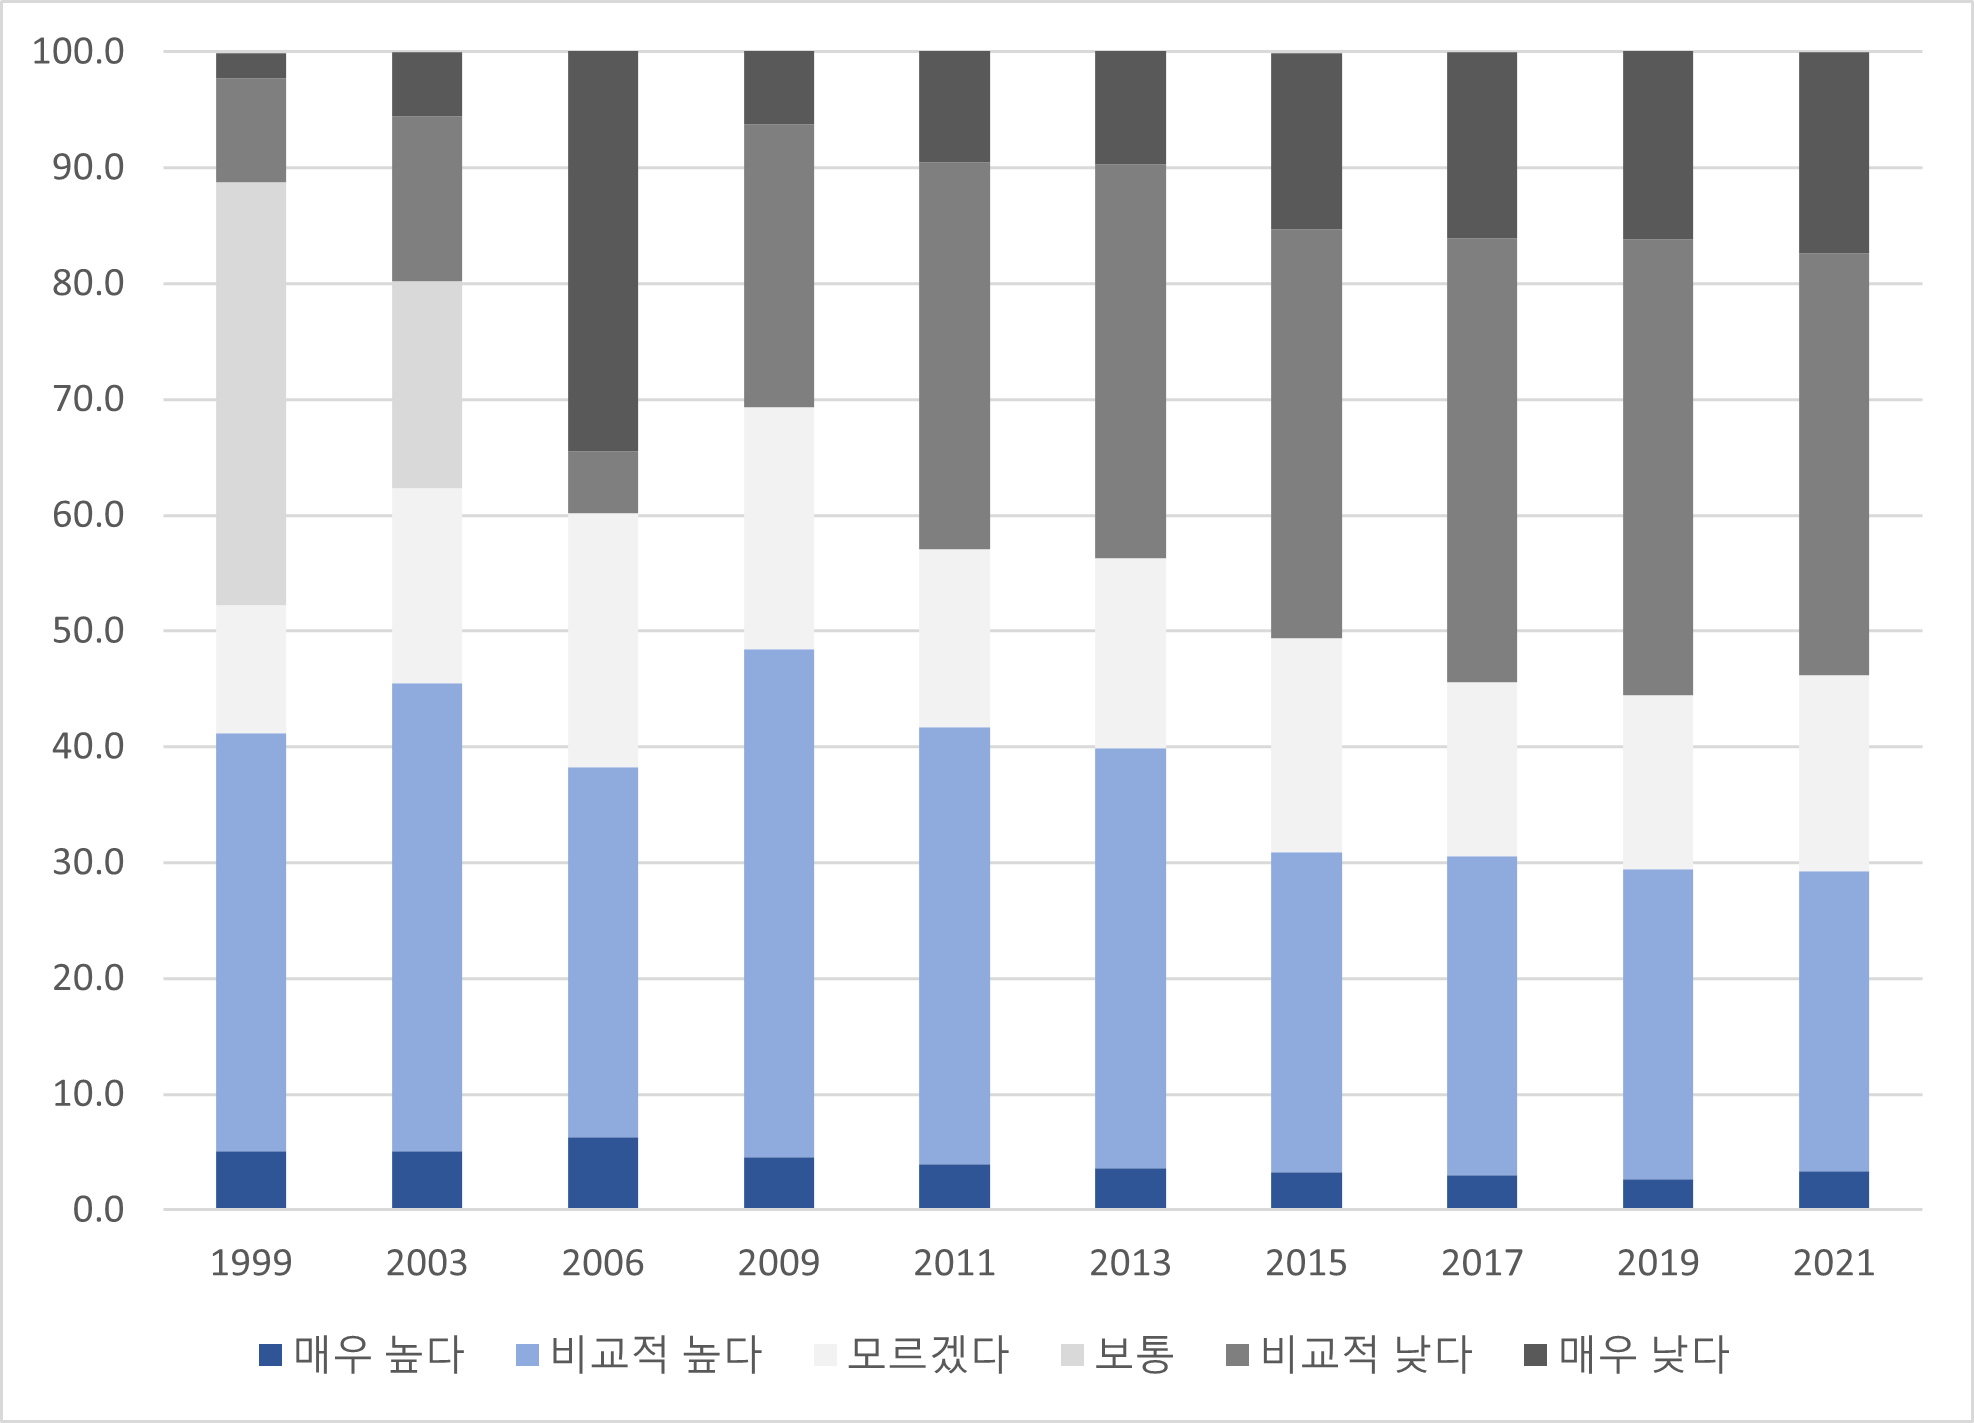
\includegraphics[width=\textwidth]{figure/kosis_intermobility_99-21.png}
        \caption{세대간 계층이동}
    \end{subfigure}
    \hfill
    \begin{subfigure}[b]{0.45\textwidth}
        \centering
        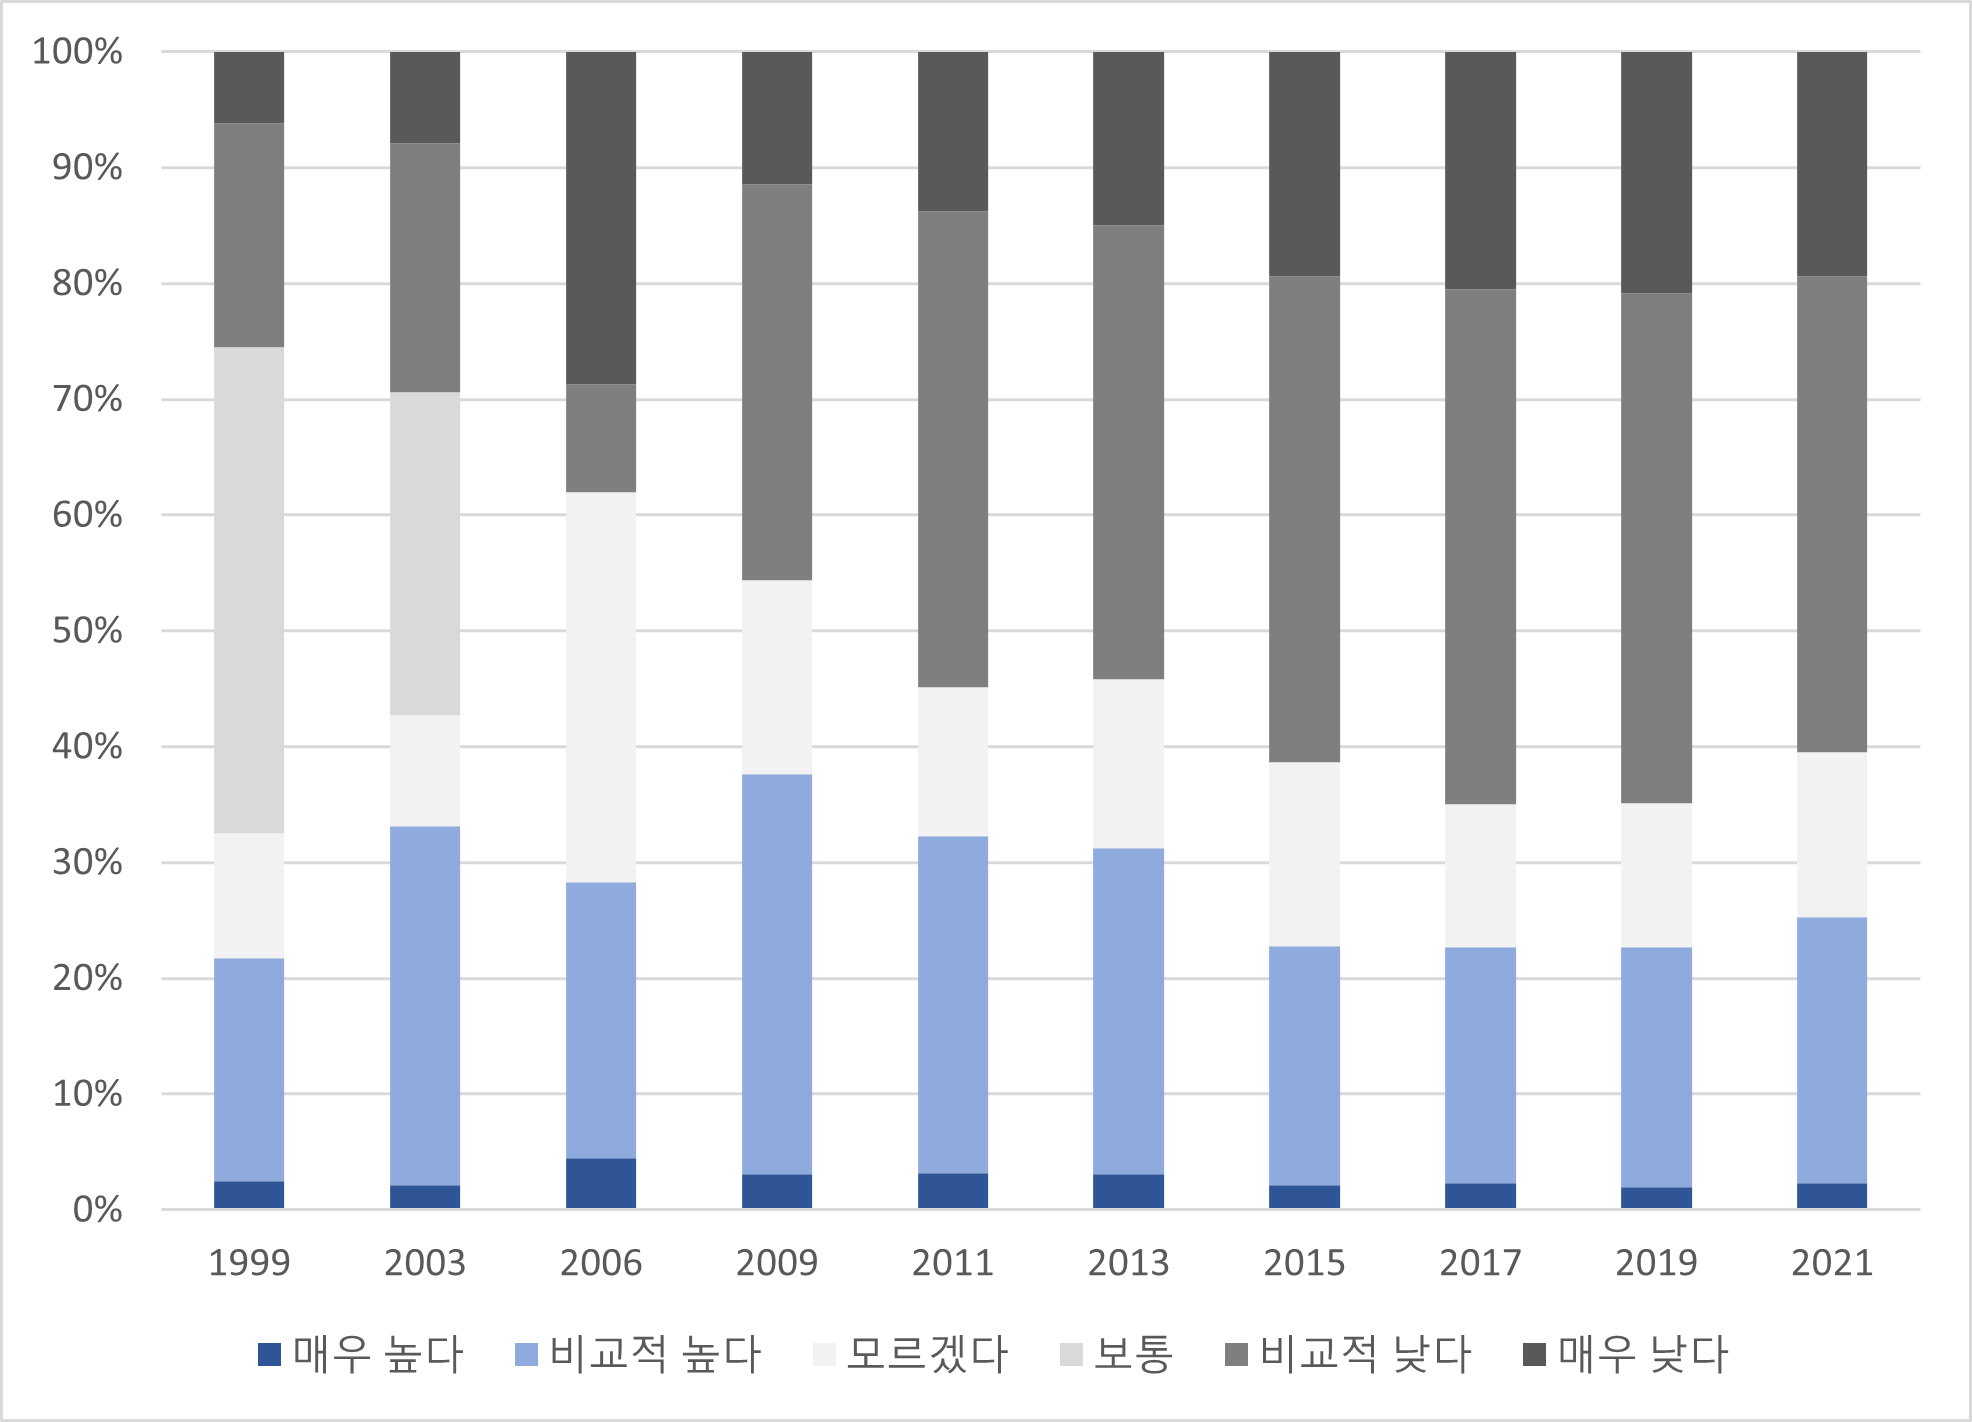
\includegraphics[width=\textwidth]{figure/kosis_intramobility_99-21.png}
        \caption{세대내 계층이동}
    \end{subfigure}
    \\
    \source{통계청, 「사회조사」, 원자료, 각 년도.}
    \label{fig:intermobility}
\end{figure}

이러한 주관적 인식의 급격한 변화와 달리 세대 간 계층이동에 대한 여러 선행연구들은 비교적 낙관적인 결론을 보였다.\footnote{한국의 지니계수 역시 2011년 0.388에서 2020년 0.331로 꾸준히 감소하여 소득분배 역시 개선되어 왔다.} \citet{cnh11}과 \citet{yang12}은 세대 간 소득탄력성(부모소득상승률에 대한 자녀소득 상승률의 비율)을 0.37이하로 추정하여 OECD국가 평균 이하었다. 이는 우리나라의 세대 간 계층이동성이 OECD 평균 보다 높은 것을 의미한다.\footnote{선행연구인 \citet{kim09}과 \citet{ketl09} 등에서는 이보다 더 낮은 탄력성이 보고되기도 하였다.}

불평등에 대한 최근의 연구는 과거와 크게 두 가지 관점에서 차이가 있다. 첫째,  불평등 연구의 대상이 부$\cdot$소득과 같은 인간행위의 결과에 머무르지 않고 이들의 주요 원인인 가정환경이나 가구소득과 같은 사회경제학적 배경을 고려한다. 다시 말해 결과의 불평등을 넘어 기회의 불평등에 초점이 맞춰지고 있다.
 
둘째, 과거에는 소득이나 부와 같은 경제적 성과에만 초점을 맞춘 불평등 문제가 대학입시제도, 특목고-자사고 축소와 같은 교육적 성취의 영역에서도 주목받고 있다. 대부분의 국가에서 교육적 성취는 개인들이 미성년기에 얻을 수 있는 가장 중요한 성취 중 하나다. 뿐만 아니라 교육적 성취는 다시 미래의 소득 획득에 중요한 요소가 된다. 따라서 교육적 성취에 대한 불평등 연구는 사회구성원이 미성년 시기에 겪는 불평등에 대한 연구와 동시에 미래의 소득불평등에 대한 원인에 대한 정보를 제공한다.

본연구의 목적은 교육과 소득이라는 생애 대표적인 두 성취에 대한 우리 사회의 기회불평등의 존재여부와 그 정도를 시계열로 제시하고 정책적 함의를 도출하는 데 있다. 우리 사회의 대다수는 성장기에 교육, 특히 대학입학를 주요 성취로 여기고 이를 달성하기 위해 매진한다. 그리고 교육과정이 끝나면 누구나 소득이나 부와 같은 경제적 성취에 매진한다. 따라서 교육 및 경제적 성취 각각을 분석함으로서 개인의 생애 전반의 성취에 대한 기회불평등 분석을 할 수 있다. 또한, 교육적 성취는 경제적 성취에 가장 중요한 설명변수다. 더 나은 교육의 성취는 두말할 나위 없이 더 나은 경제적 성취의 획득과 직결된다. 따라서 교육적 성취의 불평등에 대한 분석은 경제적 성취의 불평등을 이해하기 위해서도 중요한 자료가 된다.
 
이하의 장은 다음과 같이 구성된다.
2장에서는 대졸자직업이동경로조사(이하 GOMS)를 이용하여 2000-2011학년 고졸자의 입학대학을 성취변수로 하는 대학입학의 기회불평등과 대학졸업후 초직에서의 임금을 성취변수로 하는 경제적 기회불평등의 추이를 살펴본다. 교육적 성취의 측정에서는 수능 또는 시험점수와 같은 정량적 지표가 필요하다. 하지만 이를 공개한 전국단위의 자료는 \citet{ohetl16}에서 연구한 KEEP, KELS 두 자료가 유이하다. 그러나 두 자료는 각각 2005년 수능응시생과 2011년 수능 응시생이라는 두 코호트만을 관찰할 수 있어 교육적 성취의 기회불평등 추이를 분석할 수 없다. 반면 GOMS는 대졸자를 대상으로 조사되지만 이들의 졸업대학과 학과를 구분할 수 있어, 대학입학이라는 교육적 성취를 시계열화 하여 분석할 수 있다. 아울러 대학졸업후 초직에서 얻는 소득변수 역시 제공하여 동일한 대상에 대하여 교육적 성취와 경제적 성취를 제한적으로나마 비교분석 할 수 있다.

3장에서는 한국노동패널(이하 KLIPS)를 이용하여 1998년 이후 우리 사회 가계소득의 기회불평등 추이를 살펴본다. 2장의 자료는 대졸자를 졸업후 최장 18개월 이내에 조사하였기 때문에 경제적 기회불평등의 연구대상이 20-30대 청년으로 한정된다. 그리고 대졸자를 대상으로 하기 때문에 실제 20-30대가 겪는 실제 기회불평등보다 과소측정되는 문제가 있다. 우리 사회의 경제적 기회불평등 전체를 분석하기 위해서는 모든 개인들을 제한없이 대표하면서 소득정보 및 그들의 사회경제적 환경정보를 동시에 제공하는 자료가 필요하다. KLIPS는 이러한 조건에 부합하는 정보를 제공하여 우리 사회의 경제적 기회불평등을 시계열로 분석할 수 있게 한다.

4장에서는 연구범위와 주제를 확장한다.  주요한 두 국제 교육자료인 `수학·과학 성취도 추이변화 국제비교 연구(Trends in International Mathematics and Science Study, TIMSS)' 와 OECD 학업성취도 평가(OECD's Programme for International Student Assessment, PISA)를 이용하여 지난 20여년간 전세계 청소년의 교육성취의 기회불평등을 측정하고, 교육의 (기회)불평등이 경제성장에 어떤 영향을 주는가에 대하여 살펴본다.
5장은 이상의 연구결과에 대한 맺음글이다.